\documentclass[12pt, fullpage,letterpaper]{article}

\usepackage[margin=1in]{geometry}
\usepackage{url}
\usepackage{amsmath,amsthm,amssymb}
\usepackage{float}
\usepackage{pgfplots}
\usepgfplotslibrary{polar}
\usepgflibrary{shapes.geometric}
\usetikzlibrary{calc}
\usepackage{caption}

\pgfplotsset{my style/.append style={axis x line=middle, axis y line=
middle, xlabel={$x$}, ylabel={$y$}, axis equal }}

\newcommand{\semester}{Fall 2016}
\newcommand{\assignmentId}{5}
\newcommand{\releaseDate}{Nov 2, 2016}
\newcommand{\dueDate}{Nov 15, 2016}

\newcommand{\bx}{{\bf x}}
\newcommand{\bw}{{\bf w}}
\newcommand{\bz}{{\bf z}}
\DeclareMathOperator{\sgn}{sgn}

\title{CS 6350: Machine Learning \semester}
\author{Gopal Menon\\Homework \assignmentId}
\date{\today}

\begin{document}
\maketitle

\section{Warm up: Margins}
\label{sec:q1}

\begin{enumerate}

\item ~[5 points] Suppose we want to use an SVM to learn the XOR
  function in two dimensions. We know that XOR is not linearly
  separable, so we apply a feature transformation. In order to do so,
  we map the input $[x_1, x_2] $ into a space consisting of two
  features: $x_1$ and $x_1 x_2$. All examples are Boolean (1 for
  positive and -1 for negative) What is the maximal margin? Draw the
  separating line back in original Euclidean input space.

  \begin{table}[H]
    \centering
    \begin{tabular}{| c | c | c  |  c | }
      \hline
      $x_1$ & $x_2$  & $x_1x_2$ & $Label$ \\
      \hline
      $-1$ & $-1$ & $+1$ & $-1$\\
      $-1$ & $+1$ & $-1$ & $+1$\\
      $+1$ & $-1$ & $-1$ & $+1$\\
      $+1$ & $+1$ & $+1$ & $-1$\\
      \hline
    \end{tabular}
    \caption*{XOR Function truth table}
  \end{table}

The XOR function truth table shows the original inputs $x_1$ and $x_2$ along with the new feature $x1x2$. The label column shows $x_1 \oplus x_2$. Figure \ref{XorSvm} shows the new space with features $x_1$ and $x_1x_2$. The points in this input space are shown along with their labels. The axis for the feature $x_1$ is the linear separator with the maximum margin and is shown as the bold line. The four features in the new space become support vectors and the margin is half the distance between the lines joining the support vectors.

The input features $x_1$ and $x_2$ in the original feature space are shown in figure \ref{XorOriginal}. The lines joining the support vectors now intersect each other. The line of maximum margin in figure \ref{XorSvm} was the one where $x_1$ varied from $+\infty$ to $+\infty$ and $x_1x_2$ was $0$. The corresponding line in the original feature space would be the one where $x_1$ varies from $+\infty$ to $+\infty$ and $x_2$ is $0$, as $x_2=0$ corresponds to the case where $x_1x_2=0$ in the new feature space. This line of maximum separation is shown in bold in figure \ref{XorOriginal}.
  \begin{figure}[H]
    \centering
    \begin{tikzpicture}[domain=0:2]
      \draw[<->] (-3.2,0) -- (3.2,0) node[below right] {$x_1$};
      \draw[<->] (0,-4) -- (0,4) node[left] {$x_1x_2$};
      \draw [<->] (-3.2,3) -- (3.2,3) ;
      \draw [<->] (-3.2,-3) -- (3.2,-3) ;
      \draw [ultra thick] (-3.2,0) -- (3.2,0) ;
      \foreach \Point/\PointLabel in {(-3,3)/, (-3,-3)/, (3,-3)/, (3,3)/}
\draw[fill=black] \Point circle (0.05) node[above right] {$\PointLabel$};
\node [above] at (-3,  3) {$(-1, +1)$};
\node [below] at (-3,  3) {$ -1$};
\node [above] at (-3,  -3) {$(-1, -1)$};
\node [below] at (-3,  -3) {$ +1$};
\node [above] at (3,  -3) {$(+1, -1)$};
\node [below] at (3,  -3) {$ +1$};
\node [above] at (3,  3) {$(+1, +1)$};
\node [below] at (3,  3) {$ -1$};
    \end{tikzpicture}
    \caption{Separation of XOR function in feature space $x_1$ and $x_1x_2$.} \label{XorSvm}
  \end{figure}

  \begin{figure}[H]
    \centering
    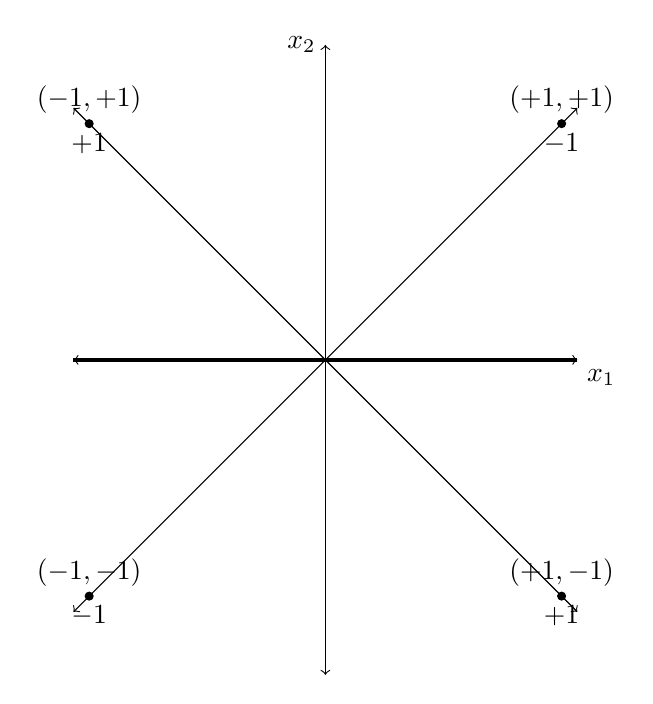
\begin{tikzpicture}[domain=0:2]
      \draw[<->] (-3.2,0) -- (3.2,0) node[below right] {$x_1$};
      \draw[<->] (0,-4) -- (0,4) node[left] {$x_2$};
      \draw [<->] (-3.2,-3.2) -- (3.2,3.2) ;
      \draw [<->] (-3.2,3.2) -- (3.2,-3.2) ;
      \draw [ultra thick] (-3.2,0) -- (3.2,0) ;
      \foreach \Point/\PointLabel in {(-3,3)/, (-3,-3)/, (3,-3)/, (3,3)/}
\draw[fill=black] \Point circle (0.05) node[above right] {$\PointLabel$};
\node [above] at (-3,  3) {$(-1, +1)$};
\node [below] at (-3,  3) {$ +1$};
\node [above] at (-3,  -3) {$(-1, -1)$};
\node [below] at (-3,  -3) {$ -1$};
\node [above] at (3,  -3) {$(+1, -1)$};
\node [below] at (3,  -3) {$ +1$};
\node [above] at (3,  3) {$(+1, +1)$};
\node [below] at (3,  3) {$ -1$};
    \end{tikzpicture}
    \caption{Separation of XOR function in original feature space $x_1$ and $x_2$.} \label{XorOriginal}
  \end{figure}
  
\item ~[10 points]  Consider the following collection of points:
  \begin{table}[H]
    \centering
    \begin{tabular}{| c | c | c  ||  c | c | c |}
      \hline
      Point & coordinate  & label & Point & coordinate  & label \\
      \hline
      $x_1$ & (0, 0)             & + & $x_5$ & (0, 1)                                & - \\
      $x_2$ & (1, 0)             & + & $x_6$ & ($\frac{1}{2}$, $\frac{\sqrt{3}}{2}$) & - \\
      $x_3$ & (1, 1)             & + & $x_7$ & ($\frac{3}{2}$, 0)                    & - \\
      $x_4$ & ($\frac{1}{2}$, 0) & + & $x_8$ & (1, $\frac{1}{2}$)                    & - \\
      \hline
    \end{tabular}
    \caption{A collection of points}
  \end{table}

  Suppose we have three training sets comprising of subsets of these
  points. We have
  $$D_1 = \{x_1, x_2, x_3, x_4, x_7\}$$
  $$D_2 = \{x_1, x_5, x_6, x_8\}$$
  $$D_3 = \{x_3, x_4, x_5, x_ 7\}$$

  \begin{enumerate}
  \item ~[6 points] Give the maximum possible margin for $D_1$, $D_2$
    and $D_3$.
   
   \begin{figure}[H]
    \centering
    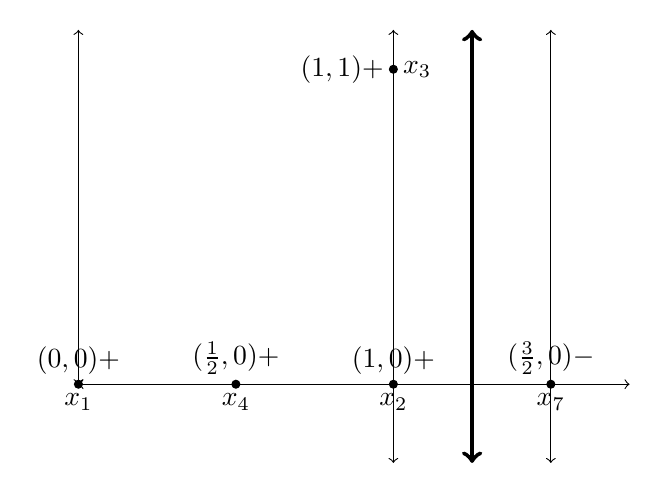
\begin{tikzpicture}[domain=0:2]
      \draw[<->] (0,0) -- (7,0);
      \draw[<->] (0,0) -- (0,4.5);
      \draw [<->] (4,-1) -- (4,4.5) ;
      \draw [<->] (6,-1) -- (6,4.5) ;
      \draw [<->] [ultra thick](5,-1) -- (5,4.5) ;
      \foreach \Point/\PointLabel in {(0,0)/, (4,0)/, (4,4)/, (2,0)/, (6,0)/}
\draw[fill=black] \Point circle (0.05) node[above right] {$\PointLabel$};
\node [above] at (0,0) {$(0,0)+$};
\node [below] at (0,0) {$x_1$};
\node [above] at (4, 0) {$(1, 0)+$};
\node [below] at (4, 0) {$x_2$};
\node [left] at (4, 4) {$(1, 1)+$};
\node [right] at (4, 4) {$x_3$};
\node [above] at (2, 0) {$(\frac{1}{2}, 0)+$};
\node [below] at (2, 0) {$x_4$};
\node [above] at (6, 0) {$(\frac{3}{2}, 0)-$};
\node [below] at (6, 0) {$x_7$};
    \end{tikzpicture}
    \caption{Points in set $D_1$.} \label{SetD1}
  \end{figure}   

The maximum margin for $D_1$ is given is shown by the solid line in figure \ref{SetD1}. This bold line is in the middle of the widest strip separating the positive and negative labels. This widest strip is shown by the two lines through $x_2$, $x_3$ and through $x_7$. The margin is thus the distance between $x_2$ and $x_7$, which is $\frac{3}{2} -1 = \frac{1}{2} =0.5$.

   
   \begin{figure}[H]
    \centering
    \begin{tikzpicture}[domain=0:2]
      \draw[<->] (-1,0) -- (10,0);
      \draw[<->] (0,-5) -- (0,4.5);
      \draw [<->] (-0.5,4.25) -- (9,-0.5) ;
      \draw [<->] (-0.5,0.25) -- (9,-4.5) ;
      \draw[] (0,0) -- (1.6,3.2);
      \draw [<->] [ultra thick](-0.5,2.25) -- (9,-2.5) ;
      \foreach \Point/\PointLabel in {(0,0)/, (0,4)/, (2,3.4641)/, (4,2)/}
\draw[fill=black] \Point circle (0.05) node[above right] {$\PointLabel$};
\node [left] at (0,0) {$(0,0)+$};
\node [below] at (0,0) {$x_1$};
\node [left] at (0, 4) {$(0, 1)-$};
\node [right] at (0, 4) {$x_5$};
\node [above] at (2, 3.4641) {$(\frac{1}{2}, \frac{\sqrt{3}}{2})-$};
\node [below] at (2, 3.4641) {$x_6$};
\node [above] at (4, 2) {$(1, \frac{1}{2})-$};
\node [below] at (4, 2) {$x_8$};
    \end{tikzpicture}
    \caption{Points in set $D_2$.} \label{SetD2}
  \end{figure}  

The widest strip separating the two labels in $D_2$ is shown in figure \ref{SetD2}, with the solid line marking the separating margin between the two labels. One side of the widest strip passes through $x_5$ and $x_8$. The slope of this line is $-\frac{1}{2}$ (computed using the formula $\frac{y_2 - y_1}{x_2 - x_1}$ for a line that passes through points $(x_1, y_1)$ and $(x_2, y_2)$). The equation of this line is $y-1=-\frac{1}{2}x$ or $x+2y=2$ (using the formula for the equation of a line that passes trough point $(x_1, y_1)$ and has a slope of $m$, which is $y-y_1 = m(x-x_1)$). The other side of the widest strip will pass through $x_1$ and will have the same slope of $-\frac{1}{2}$. So the equation of this side of the widest strip will be $x+2y=0$. The equation for the bold line separating the points with the two labels will be $x+2y=1$.

To find the width of the widest strip, we can first find the equation of the line that is perpendicular to the widest strip (slope = $2$) and passing through $(0,0)$. The equation will be $y=2x$ or $2x-y=0$. This line is shown in figure \ref{SetD2}. One end of the line is $(0,0)$ and the other end is $(0.4,0.8)$. The margin is therefore the length of this line or $\sqrt{0.4^2 + 0.8^2} = \sqrt{0.8}=0.8944$.
   
   \begin{figure}[H]
    \centering
    \begin{tikzpicture}[domain=0:2]
      \draw[<->] (0,0) -- (7,0);
      \draw[<->] (0,0) -- (0,4.5);
      \foreach \Point/\PointLabel in {(4,4)/, (2,0)/, (0,4)/,(6,0)/}
\draw[fill=black] \Point circle (0.05) node[above right] {$\PointLabel$};
\node [left] at (4, 4) {$(1, 1)+$};
\node [right] at (4, 4) {$x_3$};
\node [above] at (2, 0) {$(\frac{1}{2}, 0)+$};
\node [below] at (2, 0) {$x_4$};
\node [left] at (0, 4) {$(0, 1)-$};
\node [right] at (0, 4) {$x_5$};
\node [above] at (6, 0) {$(\frac{3}{2}, 0)-$};
\node [below] at (6, 0) {$x_7$};
    \end{tikzpicture}
    \caption{Points in set $D_3$.} \label{SetD3}
  \end{figure}   

As can be seen in figure \ref{SetD3}, the points are not linearly separable. So there os no separating margin.

  \item ~[2 points] What is the Perceptron mistake bound for these
    dataset. Which has the greatest Perceptron mistake bound.
  \item ~[2 points] Rank the datasets in terms of ``ease of
    learning''. Justify your answer.
  \end{enumerate}

\end{enumerate}


%%% Local Variables:
%%% mode: latex
%%% TeX-master: "hw"
%%% End:


\section{Kernels}
\label{sec:q2}

\begin{enumerate}  


\item  ~[15 points] If $K_1(\bx,\bz)$ and $K_2(\bx,\bz)$ are both valid kernel
  functions. In this question, you will prove that certain functions
  of kernels are valid kernels. 

  [Hint: For both the proofs below, use the the definition of a kernel
  as a dot product in a high dimensional space.]

\begin{enumerate}
\item ~[5 points] Show that the product of two kernels is a kernel.
  That is, show that $K$ in the expression below is a kernel:
  \begin{equation*}
    K(\bx,\bz) = K_1(\bx,\bz) K_2(\bx,\bz)
  \end{equation*} 

Since $K_1$ and $K_2$ are kernels, according to Mercer's condition, for every finite set $\left \{ x_1, x_2, \ldots \right \}$, for any real valued choice of $c_1, c_2, \ldots$, we have

  \begin{equation}
   \sum_i \sum_j c_i c_j K_1 \left ( \bx_i, \bx_j \right ) \geq 0
   \label{mercer1}
  \end{equation} 

  \begin{equation}
   \sum_i \sum_j c_i c_j K_2 \left ( \bx_i, \bx_j \right ) \geq 0
   \label{mercer2}
  \end{equation} 
  
  For $K_1(\bx,\bz) K_2(\bx,\bz)$ to be a Kernel, the following needs to be true
  
  \begin{equation}
   \sum_i \sum_j c_i c_j K_1 \left ( \bx_i, \bx_j \right ) K_2 \left ( \bx_i, \bx_j \right ) \geq 0
   \label{mercer3}
  \end{equation} 
  
  Let $c_j K_1 \left ( \bx_i, \bx_j \right ) =  k_j$. Since $c_j$ can take any real values, it follows that $k_j$ can take any real value. So we can now reduce the requirement of the inequality \ref{mercer3} to
  
    \begin{equation}
   \sum_i \sum_j c_i k_j K_2 \left ( \bx_i, \bx_j \right ) \geq 0
   \label{mercer4}
  \end{equation} 
  
  However requirement \ref{mercer4} is equivalent to inequality \ref{mercer2}, which is true. This means that $K_1(\bx,\bz) K_2(\bx,\bz)$ is a valid kernel.
  
\item ~[10 points] Show that a polynomial over a kernel that is
  constructed using positive coefficients is a kernel. That is, if $P$
  is any polynomial with positive coefficients, show that $K$ below is
  a kernel:
  \begin{equation*}
    K(\bx,\bz) =P( K_1(\bx,\bz))
  \end{equation*} 
Hint: You may need show  $ K(\bx,\bz) = \alpha K_1(\bx,\bz) +  \beta K_2(\bx,\bz)$ is a valid kernel and use the conclusion in the previous question.
\end{enumerate} 
  
We have already shown in the previous answer that the product of two kernels is also a kernel. That is, if $K_1(\bx, \bz)$ is a valid kernel, then $K_1(\bx, \bz)K_1(\bx, \bz)$. From this it follows that $\left(K_1(\bx, \bz)\right)^3$ is a kernel since $\left(K_1(\bx, \bz)\right)^3 = \left( K_1(\bx, \bz) K_1(\bx, \bz)\right) K_1(\bx, \bz)= K_1'(\bx, \bz)K_1(\bx, \bz)$, where 
$K_1'(\bx, \bz) =  K_1(\bx, \bz) K_1(\bx, \bz)$. We already know that $K_1'(\bx, \bz)K_1(\bx, \bz)$ is a valid kernel since its the product of two kernels. This means that 
$\left(K_1(\bx, \bz)\right)^{n+1}$ is a kernel if $\left(K_1(\bx, \bz)\right)^n$ is a kernel. Using induction we can therefore show that $\left(K_1(\bx, \bz)\right)^n$ is a kernel for any whole number $n$.\\

A polynomial over a kernel that is constructed using positive coefficients can be shown as a combination of many terms of the form $\alpha K_1(\bx, \bz) + \beta K_2(\bx, \bz) + \ldots$. Using Mercer's condition, we need to show that 

    \begin{equation}
 \sum_i \sum_j c_i k_j \left(\alpha K_1 \left ( \bx_i, \bz_j \right ) +\beta K_2 \left ( \bx_i, \bz_j \right ) + \ldots \right) \geq 0
   \label{mercer5}
  \end{equation} 

    \begin{equation}
\alpha \sum_i \sum_j c_i k_j K_1 \left ( \bx_i, \bz_j \right ) +\beta \sum_i \sum_j c_i k_j K_2 \left ( \bx_i, \bz_j \right ) + \dots  \geq 0
   \label{mercer6}
  \end{equation} 

Since $K_1(\bx, \bz)$ and $K_2(\bx, \bz)$ and other terms are kernels, and coefficients $\alpha$, $\beta$ and others are positive, relation \ref{mercer6} is true. Which means that a polynomial over a kernel that is constructed using positive coefficients is a kernel.

\item~[10 points] Given two examples $\bx \in \Re^2$ and $\bz \in
  \Re^2$, let
  \begin{equation}
    K(\bx,\bz) = 15\left(\bx^T\bz\right)^2 \exp\left(-||\bx - \bz||^2\right)
  \end{equation}
  Prove that this is a valid kernel function.
  
 \item ~(\textbf{For 6350 students})[10 points]An valid kernel can always be  expressed as inner product. Prove that the Gaussian  kernel

$$K(\bx, \bz) = \exp(\frac{-\| x -z\|^2}{2 \sigma^2})$$
 can be written down as the inner product of an feature space with infinite dimension. Hint:  You may do some expansion and  then show the middle factor can be expanded as a power series.
 


\end{enumerate}

%%% Local Variables:
%%% mode: latex
%%% TeX-master: "hw"
%%% End:


\section{Experiments}
\label{sec:q3}

In this question, you will implement the support vector machine (SVM)
and a variant of random forest which combine SVMs and decision trees.

We will use two datasets for this question:
\begin{enumerate}
\item {\tt semelion handwritten digits data}: This dataset contains
  1593 handwritten digits from around 80 persons were scanned,
  stretched in a rectangular box 16x16 in a gray scale of 256 values.
  Our goal is implement svm in this data set to determine whether is a
  number 6.
\item {\tt madelon}: This is one of five datasets used in the NIPS
  2003 feature selection challenge. There are 2000 examples in
  training set and 600 examples in test set. 
\end{enumerate}

You may reuse your code in decision tree. If \textbf{you have problems
  in decision tree}, please contact with TA to get help. You may use
Java, Python, Matlab, C/C++ for this assignment. If you want to use a
different language, you must contact the instructor first. Any other
language you may want to use \textbf{MUST} run on the CADE machines.

\subsection{Support Vector Machines}
\begin{enumerate}
\item ~[6 points] Implement SVM in handwriting dataset with hyperparameter $C=1$ and $\gamma_0 = 0.01$. Report the accuracy in test set and training set. 

\textbf{Note:}
\begin{enumerate}
\item
 update learning rate according to:
$$\gamma_t = \frac{\gamma_0}{1 +\gamma_0 *t /c}$$
in this question, as well as the following questions related to SVM.
\item
Don't forget to add bias  item as the first dimension of \textbf{x}.
\end{enumerate}

The accuracy ($\frac{TP+TN}{Number of Samples}$) obtained was

    \begin{table}[H]
    \centering
    \begin{tabular}{| c | c |}
      \hline
      Data set & Accuracy  \\
      \hline
      Test & $0.7184$\\
      \hline
      Training & $0.7240$\\
      \hline
    \end{tabular}
    \caption{Handwriting data set accuracy on test and training sets}
  \end{table}    

\item ~[8 points] Run your SVM code on the {\tt madelon} dataset and
  use 5-fold cross-validation to choose suitable parameters. At least
  attempt 6 different values for $C$ and 3 different values for
  $\gamma_0$. Report the average accuracy for each group of parameters.
  Report the accuracy in your test set as well as training set.

  Hint: You should try out $C$ in exponential steps, for example,
  $2^1, 2^{-1}, 2^{-2}, \cdots$.

\begin{longtable}{| p{.30\textwidth}  |  p{.20\textwidth} |p{.20\textwidth}  |} 
      \hline
      Starting Learning Rate $\gamma_0$& Tradeoff Value $C$ & Average Accuracy  \\
      \hline
      $10.0$ & $2.0$ & $0.4940$ \\
      \hline
      $10.0$ & $1.0$ & $0.5885$ \\
      \hline
      $10.0$ & $0.5$ & $0.5000$ \\
      \hline
      $10.0$ & $0.25$ & $0.4880$ \\
      \hline
      $10.0$ & $0.125$ & $0.5000$ \\
      \hline
      $10.0$ & $0.0625$ & $0.5000$ \\
      \hline
      $10.0$ & $0.03125$ & $0.5040$ \\
      \hline
      $10.0$ & $0.015625$ & $0.4870$ \\
      \hline
      $10.0$ & $0.0078125$ & $0.5000$ \\
      \hline
      $10.0$ & $0.00390625$ & $0.5000$ \\
      \hline
      $10.0$ & $0.001953125$ & $0.4980$ \\
      \hline
      $10.0$ & $9.765625E-4$ & $0.5000$ \\
      \hline
      $1.0$ & $2.0$ & $0.5035$ \\
      \hline
      $1.0$ & $1.0$ & $0.5655$ \\
      \hline
      $1.0$ & $0.5$ & $0.4900$ \\
      \hline
      $1.0$ & $0.25$ & $0.5020$ \\
      \hline
      $1.0$ & $0.125$ & $0.5000$ \\
      \hline
      $1.0$ & $0.0625$ & $0.5000$ \\
      \hline
      $1.0$ & $0.03125$ & $0.5000$ \\
      \hline
      $1.0$ & $0.015625$ & $0.4980$ \\
      \hline
      $1.0$ & $0.0078125$ & $0.5000$ \\
      \hline
      $1.0$ & $0.00390625$ & $0.5050$ \\
      \hline
      $1.0$ & $0.001953125$ & $0.5000$ \\
      \hline
      $1.0$ & $9.765625E-4$ & $0.5000$ \\
      \hline
      
      $0.1$ & $2.0$ & $0.5785$ \\
      \hline
      $0.1$ & $1.0$ & $0.5130$ \\
      \hline
      $0.1$ & $0.5$ & $0.5500$ \\
      \hline
      $0.1$ & $0.25$ & $0.4495$ \\
      \hline
      $0.1$ & $0.125$ & $0.5610$ \\
      \hline
      $0.1$ & $0.0625$ & $0.5010$ \\
      \hline
      $0.1$ & $0.03125$ & $0.5030$ \\
      \hline
      $0.1$ & $0.015625$ & $0.5000$ \\
      \hline
      $0.1$ & $0.0078125$ & $0.5000$ \\
      \hline
      $0.1$ & $0.00390625$ & $0.4810$ \\
      \hline
      $0.1$ & $0.001953125$ & $0.5010$ \\
      \hline
      $0.1$ & $9.765625E-4$ & $0.5050$ \\
      \hline
      
      $0.01$ & $2.0$ & $0.5285$ \\
      \hline
      $0.01$ & $1.0$ & $0.5950$ \\
      \hline
      $0.01$ & $0.5$ & $0.5105$ \\
      \hline
      $0.01$ & $0.25$ & $0.4950$ \\
      \hline
      $0.01$ & $0.125$ & $0.5695$ \\
      \hline
      $0.01$ & $0.0625$ & $0.5315$ \\
      \hline
      $0.01$ & $0.03125$ & $0.5245$ \\
      \hline
      $0.01$ & $0.015625$ & $0.5575$ \\
      \hline
      $0.01$ & $0.0078125$ & $0.5565$ \\
      \hline
      $0.01$ & $0.00390625$ & $0.5000$ \\
      \hline
      $0.01$ & $0.001953125$ & $0.5000$ \\
      \hline
      $0.01$ & $9.765625E-4$ & $0.5000$ \\
      \hline
       
      $0.001$ & $2.0$ & $0.5710$ \\
      \hline
      $0.001$ & $1.0$ & $0.5630$ \\
      \hline
      $0.001$ & $0.5$ & $0.5970$ \\
      \hline
      $0.001$ & $0.25$ & $0.5775$ \\
      \hline
      $0.001$ & $0.125$ & $0.5770$ \\
      \hline
      $0.001$ & $0.0625$ & $0.5095$ \\
      \hline
      $0.001$ & $0.03125$ & $0.4615$ \\
      \hline
      $0.001$ & $0.015625$ & $0.4775$ \\
      \hline
      $0.001$ & $0.0078125$ & $0.5545$ \\
      \hline
      $0.001$ & $0.00390625$ & $0.5310$ \\
      \hline
      $0.001$ & $0.001953125$ & $0.5000$ \\
      \hline
      $0.001$ & $9.765625E-4$ & $0.5000$ \\
      \hline
       
      $0.0001$ & $2.0$ & $0.5615$ \\
      \hline
      $0.0001$ & $1.0$ & $0.5630$ \\
      \hline
      $0.0001$ & $0.5$ & $0.5750$ \\
      \hline
      $0.0001$ & $0.25$ & $0.5770$ \\
      \hline
      $0.0001$ & $0.125$ & $0.5890$ \\
      \hline
      $0.0001$ & $0.0625$ & $0.4650$ \\
      \hline
      $0.0001$ & $0.03125$ & $0.5640$ \\
      \hline
      $0.0001$ & $0.015625$ & $0.5620$ \\
      \hline
      $0.0001$ & $0.0078125$ & $0.4875$ \\
      \hline
      $0.0001$ & $0.00390625$ & $0.4940$ \\
      \hline
      $0.0001$ & $0.001953125$ & $0.5000$ \\
      \hline
      $0.0001$ & $9.765625E-4$ & $0.4820$ \\
      \hline
       
      $0.00001$ & $2.0$ & $0.5525$ \\
      \hline
      $0.00001$ & $1.0$ & $0.5880$ \\
      \hline
      $0.00001$ & $0.5$ & $0.5820$ \\
      \hline
      $0.00001$ & $0.25$ & $0.5955$ \\
      \hline
      $0.00001$ & $0.125$ & $0.5965$ \\
      \hline
      $0.00001$ & $0.0625$ & $0.5900$ \\
      \hline
      $0.00001$ & $0.03125$ & $0.4960$ \\
      \hline
      $0.00001$ & $0.015625$ & $0.5180$ \\
      \hline
      $0.00001$ & $0.0078125$ & $0.4995$ \\
      \hline
      $0.00001$ & $0.00390625$ & $0.5000$ \\
      \hline
      $0.00001$ & $0.001953125$ & $0.5000$ \\
      \hline
      $0.00001$ & $9.765625E-4$ & $0.5000$ \\
      \hline
      
      $0.000001$ & $2.0$ & $0.5670$ \\
      \hline
      $0.000001$ & $1.0$ & $0.5880$ \\
      \hline
      $0.000001$ & $0.5$ & $0.6050$ \\
      \hline
      $0.000001$ & $0.25$ & $0.5945$ \\
      \hline
      $0.000001$ & $0.125$ & $0.5690$ \\
      \hline
      $0.000001$ & $0.0625$ & $0.4830$ \\
      \hline
      $0.000001$ & $0.03125$ & $0.4860$ \\
      \hline
      $0.000001$ & $0.015625$ & $0.4860$ \\
      \hline
      $0.000001$ & $0.0078125$ & $0.5000$ \\
      \hline
      $0.000001$ & $0.00390625$ & $0.5000$ \\
      \hline
      $0.000001$ & $0.001953125$ & $0.4860$ \\
      \hline
      $0.000001$ & $9.765625E-4$ & $0.5000$ \\
      \hline
       
      $0.0000001$ & $2.0$ & $0.5860$ \\
      \hline
      $0.0000001$ & $1.0$ & $0.5480$ \\
      \hline
      $0.0000001$ & $0.5$ & $0.5980$ \\
      \hline
      $0.0000001$ & $0.25$ & $0.5850$ \\
      \hline
      $0.0000001$ & $0.125$ & $0.4745$ \\
      \hline
      $0.0000001$ & $0.0625$ & $0.4760$ \\
      \hline
      $0.0000001$ & $0.03125$ & $0.4895$ \\
      \hline
      $0.0000001$ & $0.015625$ & $0.4870$ \\
      \hline
      $0.0000001$ & $0.0078125$ & $0.4820$ \\
      \hline
      $0.0000001$ & $0.00390625$ & $0.5000$ \\
      \hline
      $0.0000001$ & $0.001953125$ & $0.4990$ \\
      \hline
      $0.0000001$ & $9.765625E-4$ & $0.4900$ \\
      \hline
      
      $0.00000001$ & $2.0$ & $0.5420$ \\
      \hline
      $0.00000001$ & $1.0$ & $0.5925$ \\
      \hline
      $0.00000001$ & $0.5$ & $0.5465$ \\
      \hline
      $0.00000001$ & $0.25$ & $0.4955$ \\
      \hline
      $0.00000001$ & $0.125$ & $0.4810$ \\
      \hline
      $0.00000001$ & $0.0625$ & $0.4710$ \\
      \hline
      $0.00000001$ & $0.03125$ & $0.4810$ \\
      \hline
      $0.00000001$ & $0.015625$ & $0.4870$ \\
      \hline
      $0.00000001$ & $0.0078125$ & $0.4810$ \\
      \hline
      $0.00000001$ & $0.00390625$ & $0.4910$ \\
      \hline
      $0.00000001$ & $0.001953125$ & $0.5000$ \\
      \hline
      $0.00000001$ & $9.765625E-4$ & $0.4930$ \\
      \hline    
      
      $0.000000001$ & $2.0$ & $0.5210$ \\
      \hline
      $0.000000001$ & $1.0$ & $0.4920$ \\
      \hline
      $0.000000001$ & $0.5$ & $0.5010$ \\
      \hline
      $0.000000001$ & $0.25$ & $0.4880$ \\
      \hline
      $0.000000001$ & $0.125$ & $0.4850$ \\
      \hline
      $0.000000001$ & $0.0625$ & $0.4780$ \\
      \hline
      $0.000000001$ & $0.03125$ & $0.4740$ \\
      \hline
      $0.000000001$ & $0.015625$ & $0.4740$ \\
      \hline
      $0.000000001$ & $0.0078125$ & $0.4810$ \\
      \hline
      $0.000000001$ & $0.00390625$ & $0.4920$ \\
      \hline
      $0.000000001$ & $0.001953125$ & $0.4750$ \\
      \hline
      $0.000000001$ & $9.765625E-4$ & $0.4910$ \\
      \hline    
      
      
      $0.0000000001$ & $2.0$ & $0.5130$ \\
      \hline
      $0.0000000001$ & $1.0$ & $0.4930$ \\
      \hline
      $0.0000000001$ & $0.5$ & $0.4790$ \\
      \hline
      $0.0000000001$ & $0.25$ & $0.4770$ \\
      \hline
      $0.0000000001$ & $0.125$ & $0.4780$ \\
      \hline
      $0.0000000001$ & $0.0625$ & $0.4710$ \\
      \hline
      $0.0000000001$ & $0.03125$ & $0.4780$ \\
      \hline
      $0.0000000001$ & $0.015625$ & $0.4790$ \\
      \hline
      $0.0000000001$ & $0.0078125$ & $0.5065$ \\
      \hline
      $0.0000000001$ & $0.00390625$ & $0.4750$ \\
      \hline
      $0.0000000001$ & $0.001953125$ & $0.4850$ \\
      \hline
      $0.0000000001$ & $9.765625E-4$ & $0.4870$ \\
      \hline    
     \caption{Madelon data set average accuracy for hyper parameters}
  \end{longtable}  

    \begin{table}[H]
    \centering
    \begin{tabular}{| c | c |}
      \hline
      Data set & Accuracy  \\
      \hline
      Test & $0.5867$\\
      \hline
      Training & $0.6325$\\
      \hline
    \end{tabular}
    \caption{Madelon data set accuracy on test and training sets}
  \end{table}   

\item ~[6 points] Precision , recall and $ F_1$ score are another
  metrics besides accuracy, which are useful if the dataset is
  unbalanced with respect to the positive and negative examples. To
  compute these quantities, you should count the number of true
  positives (that is, examples that your classifier predicts as
  positive and are truly positive), the false positives (i.e, examples
  that your classifier predicts as positive, but are actually labeled
  negative) and the false negatives (i.e., examples that are predicted
  as negative by your classifier, but are actually positive).
  
  Denote true positives, false positive and false negative as $TP$, $FP$
  and $FN$ respectively. The precision ($p$), recall ($r$) and f-value
  $F_1$ are defined as:
  \begin{eqnarray*}
    p   & = & \frac{TP}{TP + FP} \\
    r   & = & \frac{TP}{TP+FN}   \\
    F_1 & = & 2 \frac{p \cdot r}{p + r} 
  \end{eqnarray*}

  Give precision, recall and $F_1$ score for your classifiers
  constructed in the previous two questions.

    \begin{table}[H]
    \centering
    \begin{tabular}{| c | c | c | c |}
      \hline
      Data set & Precision & Recall & $F_1$ Score  \\
      \hline
      Handwriting test& $0.6476$& $0.9967$& $0.7851$\\
      \hline
      Handwriting training& $0.6650$& $1.0000$& $0.7988$\\
      \hline
      Madelon test& $0.5802$& $0.6267$& $0.6026$\\
      \hline
      Madelon training& $0.6233$& $0.6700$& $0.6458$\\
      \hline
    \end{tabular}
    \caption{Precision, Recall and $F_1$ score for classifiers run on Handwriting and Madelon data sets}
  \end{table}   
\end{enumerate}

\subsection{Ensemble of decision trees}

Recall that a random forest is an ensemble based on bagging and
decision tree. For bagging, we draw $m$ samples {\em with replacement}
from the training set. According to
$$\lim_{m \to \infty}(1-\frac{1}{m})^m \to \frac{1}{e} \simeq 0.368$$
there are about $63.2 $ percent items may not appear that set. In
random forest, we use this sampling method $N$ times, to construct $N$
training sets and grow $N$ decision trees. Note that we build unpruned
decision trees.

In each node, instead of using the best feature by ID3 , we choose $k$
features randomly and than use the ID3 heuristic to find the best
feature to split on. Generally, $k = log_2 d $ is a good choice where d
is the number of features for our data.

Since there are $N$ trees, there will be $N$ predictions for each
example. Generally, the final prediction is voted on by these trees.
However, we would like to use SVM to combine these predictions for
this question. Specifically, after growing the $N$ decision trees, you
should construct a new $D$ consisting of transformed features. The
feature transformation $\phi(x)$ is defined using the $N$ trees as
follows:

$$\phi(x) = [tree_1(x), tree_2(x), \cdots, tree_{N} (x)]$$  

In other words, you will build an $N$ dimensional vector consisting of
the prediction (1 or -1) of each tree that you created. Thus, you have
a {\em learned} feature transformation.

You will finally train an SVM on this new dataset $D$.

\begin{enumerate}
\item ~[15 points] Using the method mentioned above, construct
  $N = 5$ decision trees for the {\tt handwriting} dataset. For each
  node, select $k = log_2 d = 8$ features randomly and then use the
  ID3 heuristic to find the best feature for splitting.

  Train the SVM meta-classifier and report the accuracy for both
  training set and test set. (No cross-validation is required but
  please choose good parameters for SVM, we will take out points for
  very low accuracy.)

\item ~[25 points] Implement same method on the {\tt madelon}
  dataset. ($k = log_2 d = 11$)
  \begin{enumerate}
  \item ~[20 points] Try $N = 10, 30, 100$. For each $N$, report
    accuracy on training set and test set. ( cross-validation is not
   required, but please choose good parameters for the SVM. )

  \item ~[5 points] Choose the best $N$ among those you have tried
    (you may try some new numbers). Report the accuracy, precision,
    recall and $f_1$ score on test set.
  \end{enumerate}
\end{enumerate}

%%% Local Variables:
%%% mode: latex
%%% TeX-master: "hw"
%%% End:



\end{document}
%%% Local Variables:
%%% mode: latex
%%% TeX-master: t
%%% End:
